\section{Generation and evaluation (Q4)}
\subsection{Generation approach (Q4.1)}
\textbf{Task fit.} We use evidence-conditioned generative question answering because questions about scientific papers may require combining methods, datasets and findings described across several passages. A generative model can synthesize this information into a coherent response, whereas a single-span extractive approach restricts the answer to a contiguous text segment.

\textbf{Relationship to established research.} Our approach follows retrieval-augmented generation: relevant passages are retrieved from an external collection and supplied as context for answer generation \citep{lewis2020rag}. This connects the answer to accessible source material rather than relying solely on knowledge stored in model parameters. PaperRAG applies this principle through its hybrid retriever and passage-level citation interface; it does not reproduce the original RAG paper's jointly trained architecture.

Work on grounded generation also distinguishes answer correctness from citation support: ALCE evaluates both, motivating our inspectable citations and separate answer-quality and grounding measurements \citep{gao2023alce}. Self-RAG learns adaptive retrieval and critique through special reflection tokens \citep{asai2023selfrag}. PaperRAG instead uses a prompted generator, a separate bounded critic and programmatic validation, without task-specific model training. This modular design lets us change retrieval and checking policies and compare their contributions while keeping the generator fixed. It trades a learned, integrated control mechanism for explicit, separately testable stages.

\textbf{Model choice.} We selected the open-weight \texttt{Qwen/Qwen3-8B} model for deployment on the available university GPU and for control over prompts, inference settings and output processing. Qwen3 supports both thinking and non-thinking modes \citep{qwen2025}; our configuration uses non-thinking generation for direct, context-conditioned answers. This is a practical model choice for the project rather than a claim that it outperforms alternative generators.

\textbf{Evidence inspection.} The generator receives retrieved passages, a closed list of citable passage IDs and an instruction to refuse when evidence is insufficient. Structured output records the answer, citations and claim provenance. Post-generation checks assess citation validity, numerical grounding and provenance consistency, making potential support issues visible to users. These checks support inspection; semantic grounding is evaluated separately through the answer-quality and RAG metrics in Q4.4--Q4.5.

\textbf{Primary evaluation configuration.}
\begin{center}\small
\begin{tabularx}{\linewidth}{lY}\toprule
Model serving & Qwen3-8B, vLLM 0.11.0, bfloat16, one NVIDIA A40 (46\,GB)\\
Decoding & Greedy (temperature 0), top-$p$ 0.9, thinking disabled; up to 1,024 new tokens\\
Context & 32,768-token model limit; up to eight passages of 1,200 characters each\\
Prompt & \texttt{p5-grounded-qa-v7}\\\bottomrule
\end{tabularx}
\end{center}

% 5/5 assessment retained internally.
% \begin{review}{Q4.1: AI-suggested five-star implementation self-check}
\draftreview{P5}{P4, P6}{P5 verifies generation choices, model/prompt settings and grounding claims; P4 checks the critic/generator boundary; P6 checks citation and report consistency.}
\colorbox{yellow!45}{\strut\textbf{DONE FOR DRAFT --- P5}}\par
Approved by Junyu Hu on 6 November 2026 for the generation approach, final serving/decoding settings and grounding description. The Qwen3-8B Hub revision remains open; P4 and P6 reviews remain pending.\par\smallskip
\aistars{3}\quad\textbf{Provisional AI assessment (7 November): 3/5 stars. Target: 5/5 --- strong implementation.} This is an editorial assessment of the current evidence, not a course grade. Lowered from 4: the handout asks for the choice to be motivated in relation to the state of the art, and this section gives only a short rationale and states that no external comparison was made. Serving, decoding and prompt settings are recorded. Two stars are withheld: P5 should add a cited comparison with alternative generation approaches, and the Qwen3-8B Hub revision is unpinned with P4/P6 reviews pending.
\end{review}


\subsection{Preprocessing (Q4.2)}
\textbf{Conservative text cleaning.} QASPER provides structured paper text, so extensive microtext normalization is unnecessary. We normalize line endings, trim surrounding whitespace and remove empty content, as described in Q1.1. We retain scientific terminology, punctuation, formulas and citation placeholders to avoid changing the meaning of the evidence. Placeholders remain as supplied by the dataset; preprocessing does not reconstruct their original contents.

\textbf{Retrieval representations.} BM25 applies case folding and word-token extraction to support lexical matching. The dense encoder uses its own tokenizer and a query-specific search instruction. These transformations prepare representations for retrieval without modifying the stored passage text shown to users. Encoder inputs are limited to 512 tokens; Q3 discusses the resulting coverage considerations.

\textbf{Generation input preparation.} Retrieved passages are rendered with their citation identifiers so that generated claims can be traced to their sources. The primary evaluation supplies at most eight passages, each limited to 1,200 characters, to bound the context supplied to the generator. The critic uses the same rendered evidence view. This preparation preserves traceability and keeps the two stages' evidence consistent. Truncation can exclude useful sentences from otherwise relevant passages; the post-hoc context-budget analysis in Section~\ref{sec:context} examines a larger 2,500-character limit.

\textbf{Output postprocessing.} Generated JSON is parsed into the answer-and-citation structure. Limited repair of invalid escape sequences handles formatting irregularities before validation. Citation and grounding checks are then applied separately; formatting repair does not establish factual correctness.

% 5/5 assessment retained internally.
% \begin{review}{Q4.2: AI-suggested five-star implementation self-check}
\draftreview{P3}{P1, P5, P4}{P3 checks corpus preprocessing; P1 checks lexical/dense transformations; P5 checks prompt rendering and output parsing; P4 verifies the clipping analysis.}
\colorbox{yellow!45}{\strut\textbf{DONE FOR DRAFT --- P1}}\par
Approved by Junlin Yin on 6 November 2026 for lexical and Dense preprocessing. Other owners' reviews remain pending.\par\smallskip
\colorbox{yellow!45}{\strut\textbf{DONE FOR DRAFT --- P5}}\par
Approved by Junyu Hu on 6 November 2026 for prompt rendering (eight passages at 1,200 characters) and structured-output parsing. Corpus preprocessing is covered by the P3 box below and the P4 review remains pending; the clipping figures (73.3\%, 33 of 45 development gold passages; 66.9\%, 232 of 347 held-out gold passages) were recomputed by P4 on the final corpus.\par\smallskip
\colorbox{yellow!45}{\strut\textbf{DONE FOR DRAFT --- P3}}\par
P3 scope: stored-text normalization and preserved source placeholders checked. Prompt clipping and parsing remain for P4/P5 verification; the clipping statistic was recomputed by P4 (73.3\%, 33 of 45 development gold passages).\par\smallskip
\aistars{5}\quad\textbf{Provisional AI assessment (7 November 2026, reassessed after preprocessing revision): 5/5 stars.} This is an editorial assessment of Q4.2 requirement coverage, not a course grade or human sign-off. The section explains why structured scientific text needs conservative cleaning rather than extensive microtext normalization. It identifies the transformations applied, the scientific content retained and the distinction between stored passages and retrieval representations. It motivates bounded generation inputs and traceable citation identifiers, explains the critic's shared evidence view, and separates JSON formatting repair from factual validation. The primary context limit and the cross-reference to post-hoc sensitivity analysis preserve the relevant experimental boundary without excessive operational detail. This directly answers whether preprocessing was needed, what was done and why. Context truncation is an explicit design trade-off, not evidence of an incomplete preprocessing answer; an additional content-preservation benchmark is not required by this item. No new experiment, corpus rebuild or owner approval is claimed. Historical owner approvals retain their original scopes.
\end{review}


\subsection{Evaluation records and annotation (Q4.3)}\label{sec:annotation}
To measure evidence recall, we locate QASPER's annotated supporting paragraphs in each paper and identify the chunks that overlap them. Matching is exact after whitespace normalization. A question is eligible only if every answer annotation has nonempty, unambiguously located evidence that the chunks fully cover. This yields 3,329 eligible questions across the official splits. We use these evidence-to-chunk mappings to measure how much of the annotated evidence the retrieval system recovers. Separately, human relevance labels assess whether retrieved passages help answer the question. QASPER reference answers are used to evaluate the generated answers.

After excluding questions recorded as used for development or chunk selection, we randomly sampled 200 unique questions from 174 papers: 78 from official validation and 122 from test. For each question, we pooled the top five passages from BM25, Dense, Hybrid RRF and Hybrid RRF + BGE rerank. After deduplication, the pool contains 1,853 unique question--passage pairs. Two annotators labelled each pair relevant or non-relevant, giving 3,706 judgments. The final labels contain 820 relevant and 1,033 non-relevant pairs (44.3\% relevant). One question has no relevant pooled passage because its candidate text replaces the requested dataset size with a formula placeholder. It remains in the evaluation, with the metric denominators stated in Section 3.2.

The revised submitted label files agree on 1,665 pairs (89.854\%), above the numerical 80\% threshold, with 188 disagreements across 109 questions. This is agreement on the current files, not a preserved measure of original independent judgments. Some batches began as AI suggestions later human-confirmed, and annotators could see which retrieval methods supplied the passages. \hyperref[tab:agreement]{Table~\ref*{tab:agreement}} also reports Cohen's kappa, which adjusts for chance agreement.

\begin{table}[htbp]\centering
\caption{Agreement on submitted labels; includes human-verified AI suggestions (Section~\ref{sec:annotation}).}\label{tab:agreement}
\begin{tabularx}{\linewidth}{YYYY}\toprule
Annotator pair & Records & Agreement & Kappa\\\midrule
Redhu / Maheshwari & 372 & 87.63\% & 0.731\\
Xu / Hu & 739 & 91.47\% & 0.791\\
Xu / Maheshwari & 191 & 94.76\% & 0.875\\
Qian / Yin & 551 & 87.48\% & 0.626\\\bottomrule\end{tabularx}\end{table}


One reviewer resolved all 188 disagreements, including 73 pairs they had originally annotated. Of these resolutions, 102 are recorded as human-reviewed and 86 as human spot-checked; the latter include 66 initially unchecked AI suggestions subsequently confirmed by the reviewer. AI suggestions may have been visible, and 176 resolutions lack written reasons. This was not independent third-person adjudication. These limits qualify the labels and agreement; the agreement percentage alone does not establish compliance with the manual-labeling requirement.

\begin{review}{Q4.3: AI-suggested five-star implementation self-check}
\draftreview{P6}{Other annotators (P1--P5)}{P3 prepares the question--passage pairs for evaluation; P6 leads result statistics, agreement analysis and annotation reporting. Every annotator confirms their own label provenance, independence and prior question exposure.}
\colorbox{yellow!45}{\strut\textbf{DONE FOR DRAFT --- P3}}\par
P3 scope: evidence mapping, exclusions, sampling, pool size, corpus identity and question--passage pair preparation. P2's statement confirms human review of all A08--10 suggestions.\par\smallskip
\aistars{3}\quad\textbf{Provisional AI assessment (7 November): 3/5 stars. Target: 5/5 --- strong implementation.} This is an editorial assessment of the current evidence, not a course grade. Pool size, agreement and kappa match the saved audit and exceed the numerical thresholds, the limitations are disclosed, and the \texttt{held\_out} sign-off was given. Two stars are withheld because resolution was neither third-person nor fully documented (176 records lack written reasons) and each annotator's own confirmation of provenance and independence is not recorded; only a team-chat confirmation of question use, relayed by P4, is on file. These numbers alone do not certify the handout's manual-labeling requirement.
\end{review}


\subsection{Answer quality (Q4.4)}
The implemented scorer uses a proposed project policy, project QA policy, version 0 (proposed), rather than the official QASPER evaluator. It lowercases text, removes ASCII punctuation and English articles, and normalizes whitespace. Exact match compares normalized strings; token F1 uses multiset token overlap. Reference extraction supports yes/no, free-form and extractive-span annotations; mixed answerability uses available answerable references.

For scientific generative answers, overlap scores can penalize correct paraphrases and reward incomplete wording. We therefore report them with refusal behavior, failures and RAG metrics rather than treating either as a complete quality measure. Relevance labels alone do not supply answer references; QA scoring also needs the linked QASPER reference answers.

Final held-out records. Job 51585 produced 200 records for each arm. Under the project QA policy, static answered 194 questions, refused 4 and failed 2; adaptive answered 191, refused 7 and failed 2; static-wide answered 194, refused 4 and failed 2. The two failures per arm are responses downgraded after a parse error; the P5 status count records them as refusals. All 200 held-out questions have at least one answerable QASPER reference annotation, so the unanswerable subset is empty. Exact match is 0.005 for every arm; token F1 is 0.368 (static), 0.366 (adaptive) and 0.368 (static-wide). On the 160 questions P4 did not annotate, F1 is 0.369 for both static and adaptive. The point estimates show no adaptive answer-quality gain.
\begin{table}[htbp]\centering\small
\caption{Final QA on the 200 held-out questions under the project policy \texttt{p6-qa-v0-proposed}. Coverage is answered questions over the subset; parse-error failures are not counted as answered.}\label{tab:qa}
\begin{tabularx}{\linewidth}{>{\hsize=1.8\hsize\linewidth=\hsize}Y>{\hsize=0.8\hsize\linewidth=\hsize}Y>{\hsize=0.8\hsize\linewidth=\hsize}Y>{\hsize=0.8\hsize\linewidth=\hsize}Y>{\hsize=0.8\hsize\linewidth=\hsize}Y}\toprule
Arm / subset & EM & Token F1 & Unanswerable correct & Coverage\\\midrule
Static / all 200 & 0.005 & 0.368 & n/a & 194/200 (0.970)\\
Adaptive / all 200 & 0.005 & 0.366 & n/a & 191/200 (0.955)\\
Static / remaining 160 & 0.006 & 0.369 & n/a & 155/160 (0.969)\\
Adaptive / remaining 160 & 0.006 & 0.369 & n/a & 152/160 (0.950)\\\bottomrule\end{tabularx}
\end{table}
\begin{review}{Final QA run}
Scores above use job 51585 and P3's \texttt{qa.jsonl} (SHA-256 \texttt{1515fc58...}), rerun with the \texttt{held\_out} role after the team sign-off of 6 November; the numbers did not change. Paired uncertainty is in Section~\ref{sec:agent-heldout}. The agent developer saw 40 evaluation questions while annotating, hence both all 200 and the remaining 160. The review file \texttt{results/final/p4/held-out/review/final-evaluation-review.json} records, as relayed by P4, that every member confirmed no held-out question was used beyond reading it for annotation. Every question was still read by its annotators, so do not call the 160 independently held out.
\end{review}

\begin{review}{Q4.4: AI-suggested five-star implementation self-check}
\draftreview{P5}{P4, P3, P6}{P5 verifies answer files and QA scores; P4 checks paired arms and the exposure subset; P3 checks references and question IDs; P6 cross-checks scorer policy, coverage and tables.}
\colorbox{yellow!45}{\strut\textbf{DONE FOR DRAFT --- P5}}\par
Approved by Junyu Hu on 6 November 2026 for the scorer policy, the final answer/refusal records and the held-out QA scores. P4/P3/P6 reviews remain open.\par\smallskip
\aistars{4}\quad\textbf{Provisional AI assessment (7 November): 4/5 stars. Target: 5/5 --- strong implementation.} This is an editorial assessment of the current evidence, not a course grade. Final EM and token F1 are reported for all 200 and the remaining 160 with answered/refused/failed counts, coverage, paired paper-level intervals and the \texttt{held\_out} role; all figures match the saved outputs. One star is withheld: the held-out list has no unanswerable question, overlap scoring cannot judge paraphrases and no human answer sample was read, and the P4/P3/P6 reviews are pending.
\end{review}


\subsection{Answer-level RAG metrics (Q4.5)}
RAGAS \citep{es2024ragas} complements overlap scoring with judgments about grounding and relevance. The project runs RAGAS 0.2.15 with a live judge. Faithfulness asks whether answer claims are supported by the supplied contexts; response relevance asks whether the answer addresses the question; context precision assesses the usefulness and ordering of retrieved contexts. The judge scores the exact rendered contexts (8 passages x 1,200 characters), not the full retrieved chunks.
\begin{table}[htbp]\centering\small
\caption{Live RAGAS on the 200 held-out questions; values are means with valid-score counts. Refusals and parse-error failures are excluded from each denominator.}\label{tab:ragas}
\begin{tabularx}{\linewidth}{YYYY}\toprule
Arm & Faithfulness & Response relevance & Context precision\\\midrule
Static & 0.892 (194) & 0.854 (193) & 0.578 (194)\\
Adaptive & 0.907 (191) & 0.854 (189) & 0.577 (191)\\\bottomrule\end{tabularx}
\end{table}
Live judge. On 6 November 2026 the rendered contexts were scored with \texttt{qwen-plus-2025-12-01} as the judge and \texttt{qwen3.7-text-embedding} for response relevance, both through DashScope's OpenAI-compatible endpoint (timeout 120 s, one worker, no automatic retries). One static and two adaptive response-relevance scores were invalid. Paired differences over the 188--191 questions scored in both arms are $+0.012$ (95\% interval $-0.001$ to $0.026$) for faithfulness, $-0.003$ ($-0.008$ to $0.001$) for response relevance and $-0.002$ ($-0.015$ to $0.010$) for context precision (1,000 paper-cluster bootstrap resamples, seed 42). The intervals do not support an adaptive advantage. Judge scores are model judgments, not human verification.
\begin{review}{RAGAS prerequisites}
Record the judge \texttt{qwen-plus-2025-12-01}, embedding \texttt{qwen3.7-text-embedding}, DashScope endpoint, timeout, concurrency and retry policy. DashScope's embeddings endpoint requires \texttt{check\_embedding\_ctx\_length=False}; without it response relevance fails with a bad request, so the runner wrapper sets it. Valid-score counts are in the table; refusals, parse errors and invalid scores are excluded. These outputs still carry the \texttt{development} role label. Review a sample manually and confirm that the judge measures the intended property; P6's evaluator review remains pending.
\end{review}

\begin{review}{Q4.5: AI-suggested five-star implementation self-check}
\draftreview{P5}{P6}{Following the evaluation handoff, P5 supplies exact contexts and verifies the RAGAS run/results; P6 checks evaluator configuration, metric interpretation, valid-score counts and reporting.}
\colorbox{yellow!45}{\strut\textbf{DONE FOR DRAFT --- P5}}\par
Approved by Junyu Hu on 6 November 2026 for the live RAGAS run, judge configuration and metric interpretation. The DashScope embedding wrapper and P6's evaluator review remain open.\par\smallskip
\aistars{1}\quad\textbf{Provisional AI assessment: 1/5 stars. Target: 5/5 --- strong implementation.} This is an editorial assessment of the current evidence, not a course grade. The RAGAS runner exists and live scores are now available for static and adaptive. Confirm the judge and embedding backends, metric definitions and budget, and keep valid-score counts, exclusions and invalid scores with the means. Review a sample manually to assess whether the judge is measuring the intended property.
\end{review}


\subsection{Latency, cost and scaling (Q4.6)}
End-to-end timing comes from two settings that must not be combined: the five-query demonstration in Q2.2 (school GPU, all papers, one pass) and the frozen held-out run on one A40 reported below (1{,}200 characters, 200 questions per arm). Their laptop predecessors in Q2.2 used a different model. Historical retrieval measurements on 100 training questions and the older 200/40 corpus report RRF p50/p95 of 17.57/21.34 ms versus 2,387.34/3,768.72 ms with BGE reranking. Those measurements include first-use costs and three empty results, without warm-up; they exclude setup outside retrieval calls. They should not be combined with the Q2.2 timings or interpreted as a controlled final speedup.

Per-paper exact search depends mainly on the selected paper's passages. All-papers exact vector search grows with the indexed corpus. The current service permits one active answer request and returns HTTP 429 when busy; serial demonstration throughput does not establish concurrent capacity. Local and university model serving avoids per-call API charges, but compute and energy are not free. The paid judge cost is reported below.

Final generation timing. In job 51585, answer generation on one A40 (warm engine, serial calls) had p50/p95 latency of 10.5/23.6\,s for static, 11.1/24.0\,s for adaptive and 10.5/22.2\,s for static-wide (200 questions per arm, all records; generation only, excluding model load and, for adaptive, the agent loop). The agent loop added a mean 5.6\,s per adaptive question (p95 12.3\,s). The job completed 600 arm-question records in 2\,h\,23\,min. These are observed serial timings, not a controlled throughput benchmark; startup, concurrency and cache effects remain to be measured.
\begin{review}{Final performance measurements}
Wall time, counts, percentiles and judge cost are reported below. Startup and concurrent load remain unmeasured. The generation-only static p50 above (10.5\,s) and the end-to-end static p50 in \hyperref[tab:perf]{Table~\ref*{tab:perf}} (10.6\,s) now agree, the 0.04\,s difference being retrieval time: both cover all 200 records per arm, including the two answers the validator downgraded after a parse error. The 10.1\,s in an earlier version was computed over the 198 records without them, and the two downgraded answers are among the slowest, so excluding them lowered the median. Historical cluster timings summarized in the workbook lack raw local records and are not used here as final benchmark results.
\end{review}

End-to-end timing comes from the frozen held-out run (job 51585): 200 questions per arm, one NVIDIA A40, Qwen3-8B in bfloat16 through vLLM 0.11.0, retrieval on CPU, one request at a time with the engine warm and no score cache. Latency is agent time plus generation time per question; throughput divides the questions by the wall-clock time the runner measured for each arm, not by summed latencies (\hyperref[tab:perf]{Table~\ref*{tab:perf}}). Percentiles are over all 200 records per arm, including the two answers per arm that the validator downgraded after a parse error, which are among the slowest (about 33\,s of generation each).
\begin{table}[htbp]\centering\small
\caption{Held-out end-to-end performance, 200 questions per arm, serial requests on one A40. Percentiles are over all 200 records per arm. Tokens are the generator's totals.}\label{tab:perf}
\small\begin{tabularx}{\linewidth}{>{\hsize=1.9\hsize\linewidth=\hsize}Y>{\hsize=0.85\hsize\linewidth=\hsize}Y>{\hsize=0.85\hsize\linewidth=\hsize}Y>{\hsize=0.85\hsize\linewidth=\hsize}Y>{\hsize=0.85\hsize\linewidth=\hsize}Y>{\hsize=0.85\hsize\linewidth=\hsize}Y>{\hsize=0.85\hsize\linewidth=\hsize}Y}\toprule
Arm & Wall time (s) & Questions\newline /s & p50 (s) & p95 (s) & Prompt tokens & Output tokens\\\midrule
Static (8 passages) & 2{,}519 & 0.079 & 10.6 & 23.7 & 934{,}334 & 73{,}586\\
Adaptive & 3{,}583 & 0.056 & 16.5 & 32.9 & 928{,}803 & 74{,}598\\
Static-wide (15 passages) & 2{,}456 & 0.081 & 10.6 & 22.3 & 934{,}460 & 73{,}573\\\bottomrule\end{tabularx}
\end{table}
\begin{figure}[htbp]\centering
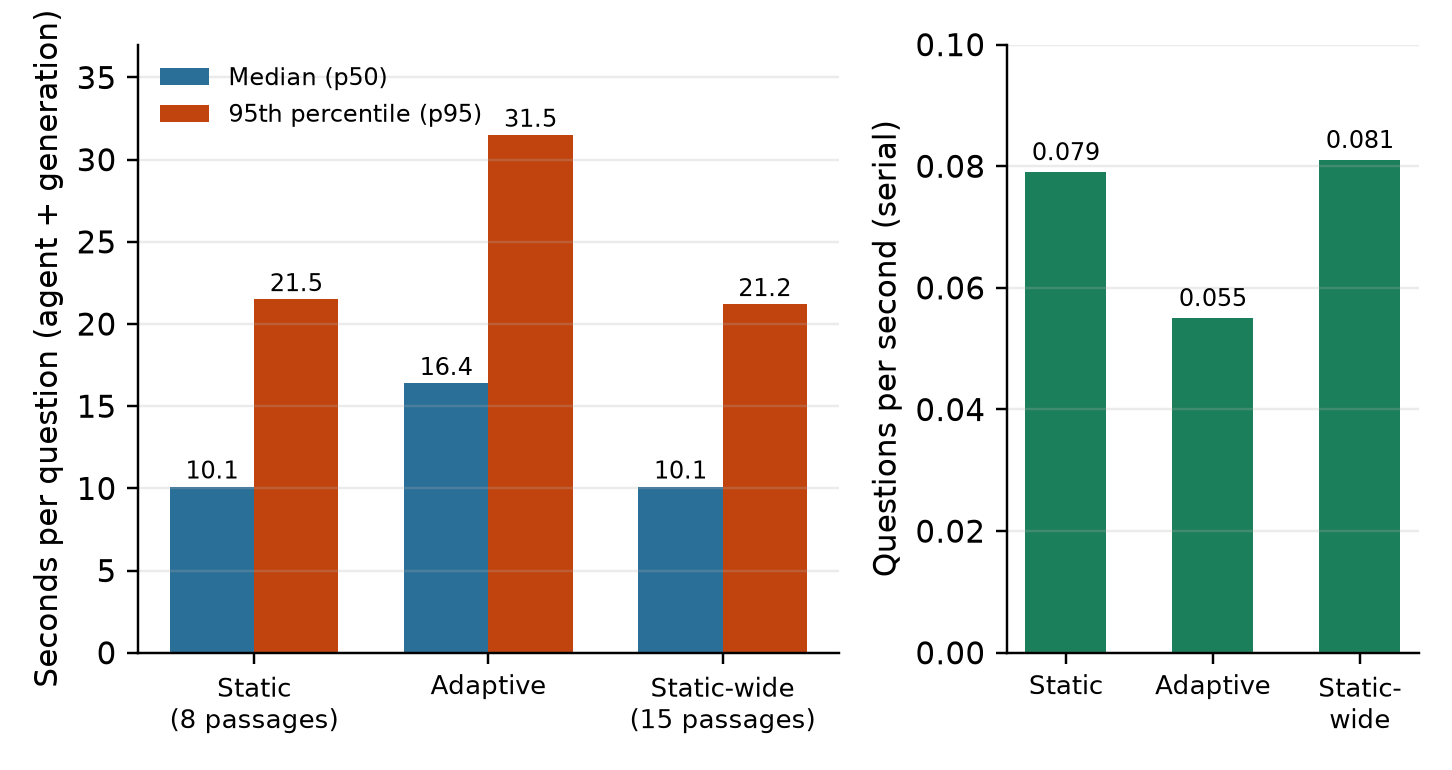
\includegraphics[width=0.92\linewidth]{images/latency-by-arm.png}
\caption{Held-out latency per question (left; agent plus generation time, one A40, serial requests) and throughput (right) by arm, the values of \hyperref[tab:perf]{Table~\ref*{tab:perf}}. The retry loop raises median latency by about 56\% and lowers throughput by about 30\%.}\label{fig:latency}
\end{figure}
Generation dominates: retrieval and fusion take 0.04\,s per question on the cluster CPU, against about 12\,s for the answer. The agent loop adds a mean 5.6\,s per question, 251 critic calls over 200 questions, and raises median latency by about 56\% (16.5 against 10.6\,s) and lowers throughput by about 30\%, for a recall gain of 0.013 (Section~\ref{sec:agent-heldout}). The critic's own token use was not recorded, so the adaptive arm's token total is a lower bound. There is no per-call monetary cost, because the model is served locally; GPU time was 2\,h 23\,min for the three arms. The RAGAS judge (Q4.5) was a paid hosted model: scoring the two arms took about 2.5 hours and cost about 0.63 Singapore dollars, as reported by the member who ran it. Concurrent throughput was not measured: calls were serial, and these figures are not a scaling benchmark.

\begin{review}{Q4.6: AI-suggested five-star implementation self-check}
\draftreview{P4}{P5, P6, P1, P2}{Following the evaluation handoff, P4 verifies final agent timing and cost; P5 checks GPU/model records; P6 verifies local UI timings and calculations; P1/P2 check historical retrieval measurements.}
\colorbox{yellow!45}{\strut\textbf{DONE FOR DRAFT --- P1}}\par
Approved by Junlin Yin on 6 November 2026 for the source attribution and wording of historical retrieval measurements. This approval does not certify a timing rerun or final GPU performance. Other owners' reviews remain pending.\par\smallskip
\colorbox{yellow!45}{\strut\textbf{DONE FOR DRAFT --- P5}}\par
Approved by Junyu Hu on 6 November 2026 for the model/GPU record and the final generation timings. P4's end-to-end benchmark and P6's local timing review remain pending.\par\smallskip
\aistars{3}\quad\textbf{Provisional AI assessment (7 November 2026, post-review): 3/5 stars.} This is an editorial assessment of the documented evidence, not a course grade or human sign-off. The report separates demonstration, historical retrieval, generation-only and end-to-end timings and supplies hardware, serial-request boundaries, percentiles, throughput, failures, generator tokens and reported judge cost. It discloses missing critic tokens and avoids a concurrency claim. Generation-only and end-to-end medians are now computed over the same 200 records with one percentile convention and agree. Startup, concurrent load and repeated-run variability are unmeasured, so the results describe observed serial performance rather than a scaling benchmark.
\end{review}

